\documentclass[tikz,border=8pt]{standalone}
\usepackage{amsmath}
\usetikzlibrary{shapes.geometric,arrows.meta,positioning,fit,backgrounds}

\begin{document}
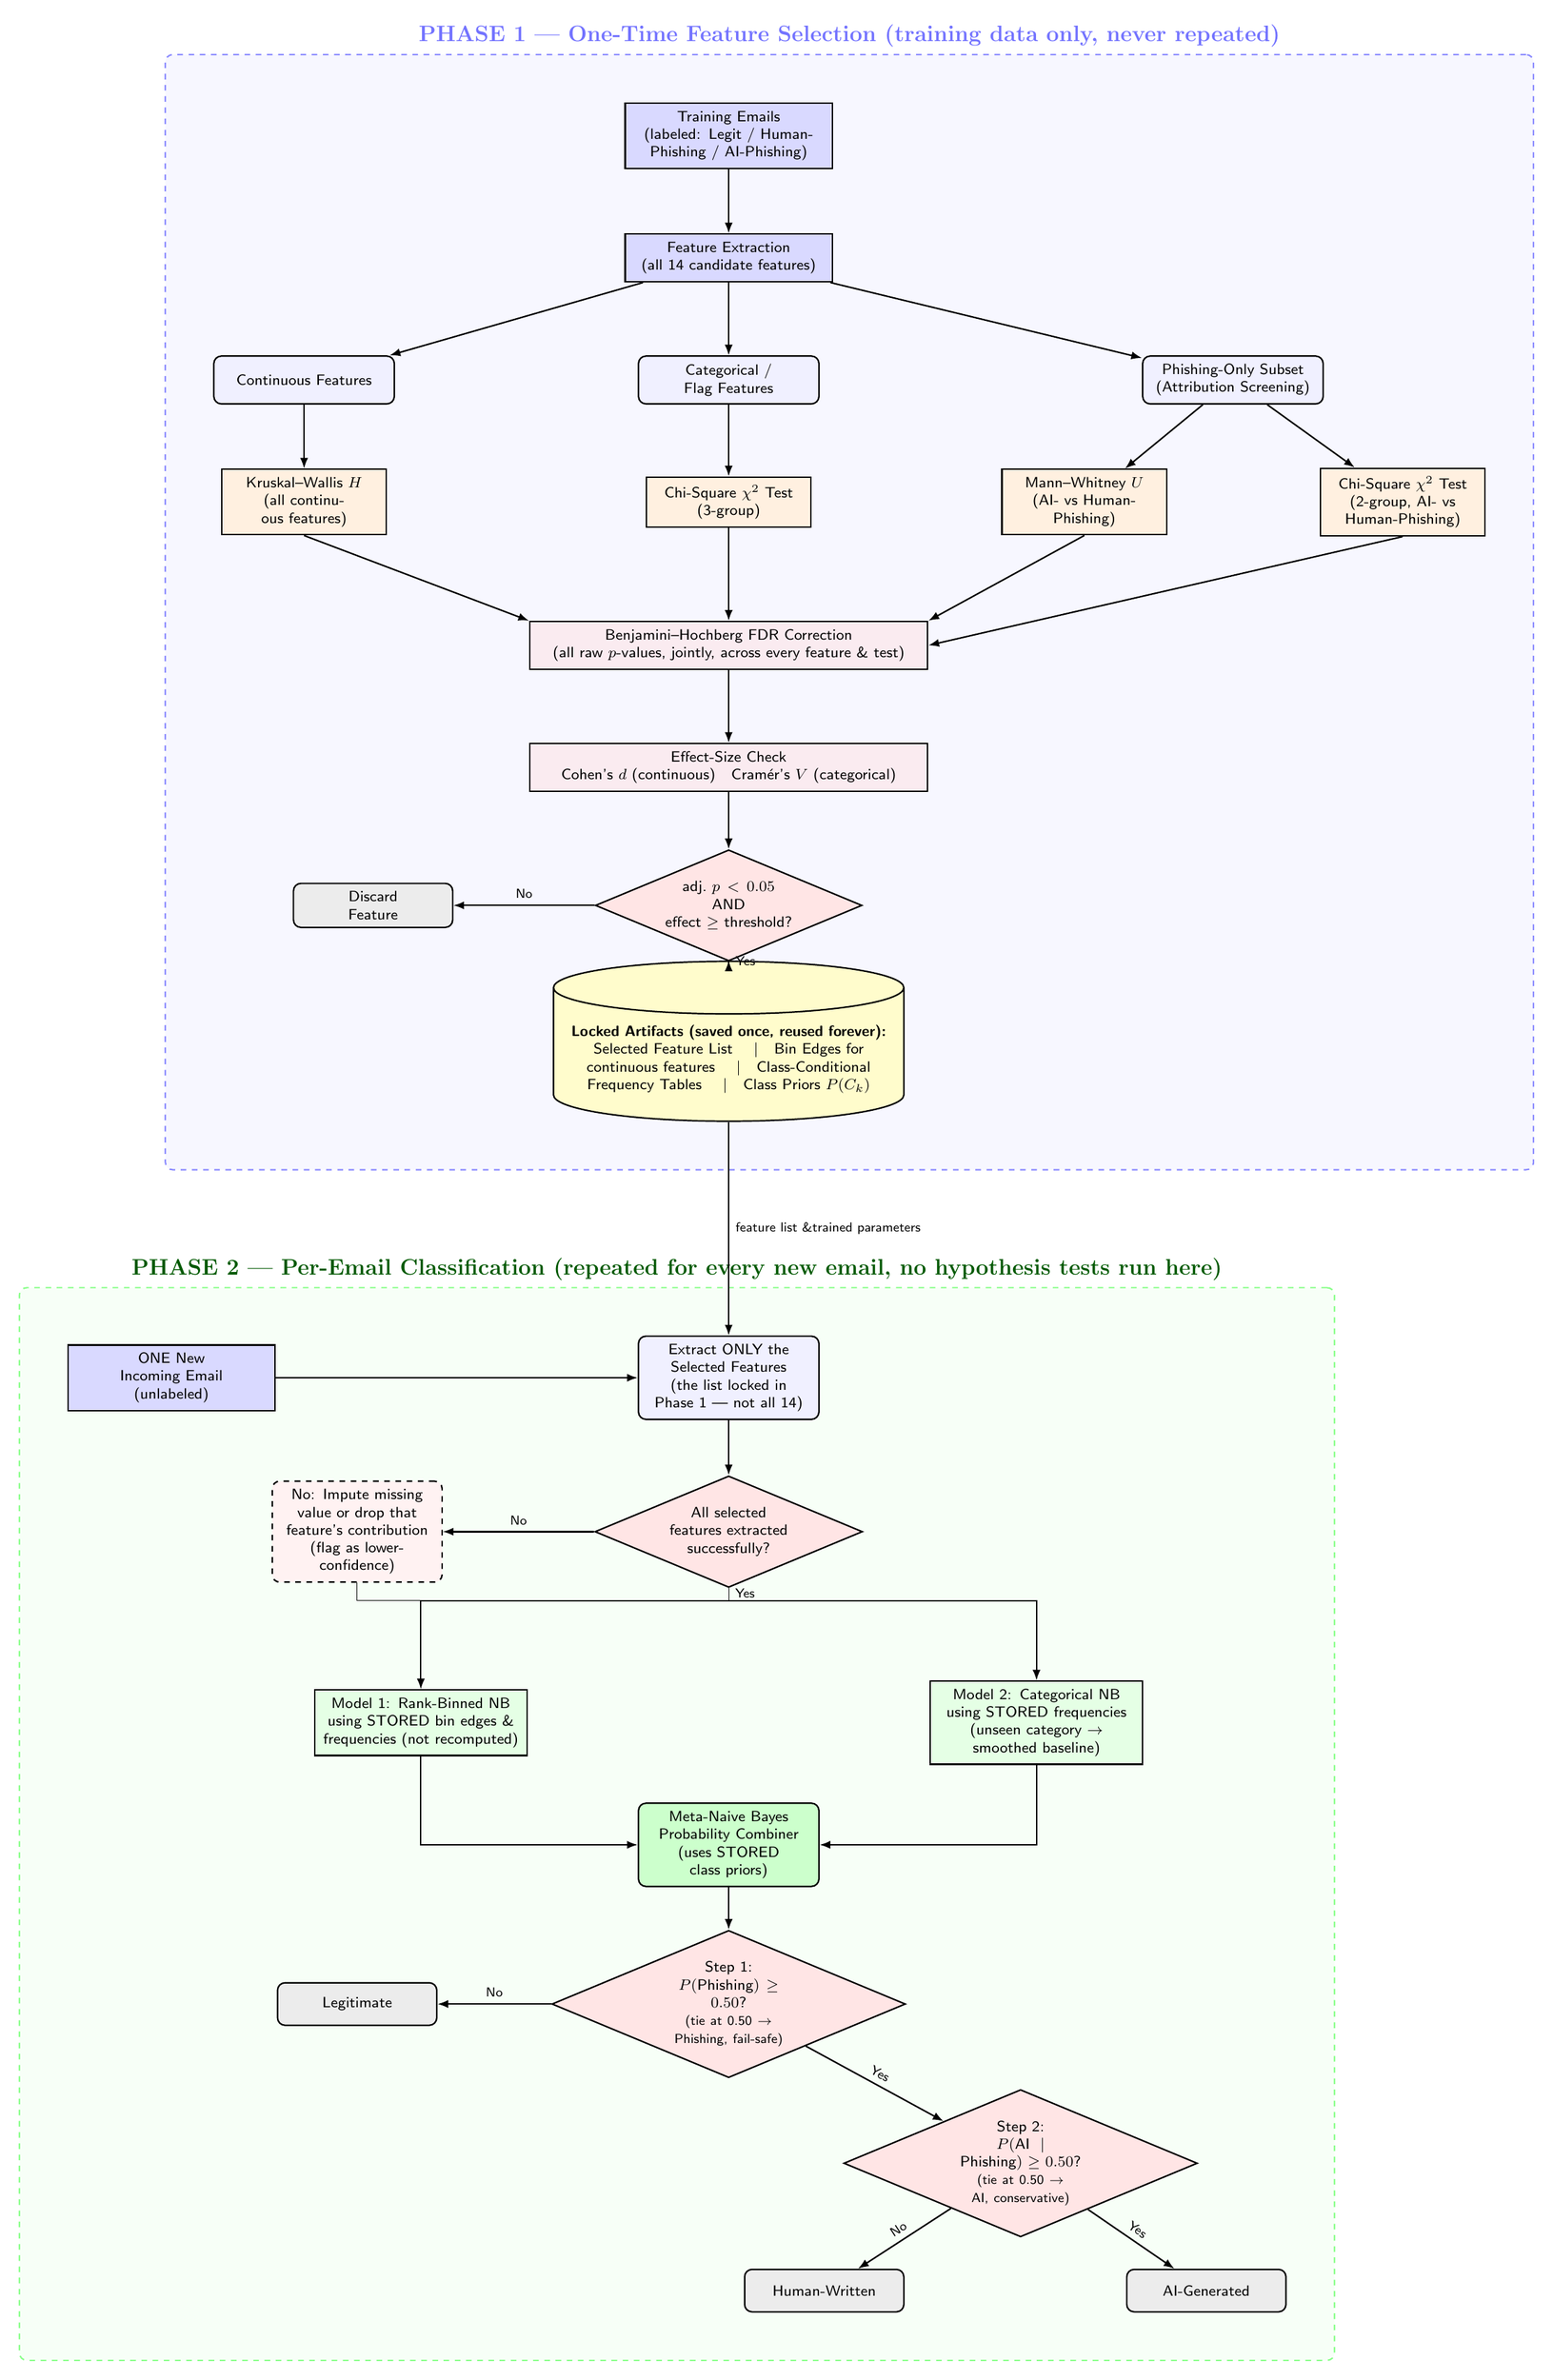
\begin{tikzpicture}[
    font=\sffamily\footnotesize,
    box/.style={rectangle, draw, thick, rounded corners, fill=blue!6,
                minimum height=0.9cm, text width=3.1cm, align=center, inner sep=1.5mm},
    io/.style={rectangle, draw, thick, fill=blue!15,
               minimum height=0.9cm, text width=3.6cm, align=center, inner sep=1.5mm},
    test/.style={rectangle, draw, thick, fill=orange!12,
                 minimum height=0.9cm, text width=2.8cm, align=center, inner sep=1.5mm},
    gate/.style={diamond, draw, thick, fill=red!10, aspect=2.4,
                 text width=2.5cm, align=center, inner sep=0.5mm},
    model/.style={rectangle, draw, thick, fill=green!10,
                  minimum height=1.0cm, text width=3.7cm, align=center, inner sep=1.5mm},
    term/.style={rectangle, draw, thick, rounded corners, fill=gray!15,
                 minimum height=0.8cm, text width=2.7cm, align=center, inner sep=1.5mm},
    conv/.style={rectangle, draw, thick, fill=purple!8,
                 minimum height=0.9cm, text width=7.2cm, align=center, inner sep=1.5mm},
    store/.style={cylinder, draw, thick, fill=yellow!20, shape border rotate=90,
                  aspect=0.15, text width=6.2cm, align=center, inner sep=2mm,
                  minimum height=1.6cm},
    err/.style={rectangle, draw, thick, dashed, rounded corners, fill=red!5,
                text width=2.9cm, align=center, inner sep=1.5mm},
    lbl/.style={font=\sffamily\scriptsize},
    arr/.style={-{Latex[length=2mm]}, thick},
]

% =====================================================================
% PHASE 1 — ONE-TIME FEATURE SELECTION (runs once, on the training set)
% =====================================================================
\node[io] (input) at (0,0) {Training Emails\\(labeled: Legit / Human-Phishing / AI-Phishing)};
\node[io] (extract) at (0,-2.3) {Feature Extraction\\(all 14 candidate features)};
\draw[arr] (input) -- (extract);

\node[box] (contlane) at (-8,-4.6)   {Continuous Features};
\node[box] (catlane)  at (0,-4.6)    {Categorical / Flag Features};
\node[box] (attrlane) at (9.5,-4.6)  {Phishing-Only Subset\\(Attribution Screening)};
\draw[arr] (extract) -- (contlane);
\draw[arr] (extract) -- (catlane);
\draw[arr] (extract) -- (attrlane);

\node[test] (kw)     at (-8,-6.9)   {Kruskal--Wallis $H$\\(all continuous features)};
\node[test] (chisq3) at (0,-6.9)    {Chi-Square $\chi^2$ Test\\(3-group)};
\node[test] (mwu)    at (6.7,-6.9)  {Mann--Whitney $U$\\(AI- vs Human-Phishing)};
\node[test] (chisq2) at (12.7,-6.9) {Chi-Square $\chi^2$ Test\\(2-group, AI- vs\\ Human-Phishing)};
\draw[arr] (contlane) -- (kw);
\draw[arr] (catlane) -- (chisq3);
\draw[arr] (attrlane) -- (mwu);
\draw[arr] (attrlane) -- (chisq2);

\node[conv] (fdr) at (0,-9.6) {Benjamini--Hochberg FDR Correction\\(all raw $p$-values, jointly, across every feature \& test)};
\draw[arr] (kw.south) -- (fdr.north west);
\draw[arr] (chisq3.south) -- (fdr.north);
\draw[arr] (mwu.south) -- (fdr.north east);
\draw[arr] (chisq2.south) -- (fdr.east);

\node[conv] (effsize) at (0,-11.9) {Effect-Size Check\\Cohen's $d$ (continuous)\quad Cram\'er's $V$ (categorical)};
\draw[arr] (fdr) -- (effsize);

\node[gate] (gateQ) at (0,-14.5) {adj.\ $p<0.05$\\AND\\effect $\geq$ threshold?};
\draw[arr] (effsize) -- (gateQ);

\node[term] (discard) at (-6.7,-14.5) {Discard\\Feature};
\draw[arr] (gateQ) -- node[lbl,above]{No} (discard);

\node[store] (storage) at (0,-17.4) {\textbf{Locked Artifacts (saved once, reused forever):}\\
Selected Feature List \quad$\vert$\quad Bin Edges for continuous features \quad$\vert$\quad
Class-Conditional Frequency Tables \quad$\vert$\quad Class Priors $P(C_k)$};
\draw[arr] (gateQ.south) -- node[lbl,right]{Yes} (storage.north);

\begin{pgfonlayer}{background}
\node[draw=blue!45, thick, dashed, rounded corners, fill=blue!3,
      fit=(input)(extract)(contlane)(catlane)(attrlane)(kw)(chisq3)(mwu)(chisq2)(fdr)(effsize)(gateQ)(discard)(storage),
      inner sep=9mm,
      label={[blue!55,font=\bfseries\large]above:PHASE 1 --- One-Time Feature Selection (training data only, never repeated)}]
      (phase1box) {};
\end{pgfonlayer}

% =====================================================================
% PHASE 2 — PER-EMAIL CLASSIFICATION (runs every time, on one new email)
% =====================================================================
\node[io] (newemail) at (-10.5,-23.4) {ONE New\\Incoming Email\\(unlabeled)};
\node[box] (extract2) at (0,-23.4) {Extract ONLY the Selected Features\\(the list locked in Phase 1 --- not all 14)};
\draw[arr] (storage.south) -- node[lbl,right]{feature list \&\\ trained parameters} (extract2.north);
\draw[arr] (newemail) -- (extract2);

\node[gate] (extractOK) at (0,-26.3) {All selected\\features extracted\\successfully?};
\draw[arr] (extract2) -- (extractOK);

\node[err] (impute) at (-7,-26.3) {No: Impute missing value or drop that feature's contribution\\(flag as lower-confidence)};
\draw[arr] (extractOK) -- node[lbl,above]{No} (impute);

\node[model] (rbnb2) at (-5.8,-29.9) {Model 1: Rank-Binned NB\\using STORED bin edges \& frequencies (not recomputed)};
\node[model] (cnb2)  at (5.8,-29.9)  {Model 2: Categorical NB\\using STORED frequencies\\(unseen category $\rightarrow$ smoothed baseline)};

% Both the "Yes" path and the impute fallback merge into ONE trunk before
% fanning out — avoids the two paths overlapping each other's lines.
\coordinate (merge) at (0,-27.6);
\draw (extractOK.south) -- node[lbl,right,pos=0.4]{Yes} (merge);
\draw (impute.south) |- (merge);
\draw[arr] (merge) -| (rbnb2.north);
\draw[arr] (merge) -| (cnb2.north);

\node[box, fill=green!20] (meta2) at (0,-32.2) {Meta-Naive Bayes\\Probability Combiner\\(uses STORED class priors)};
\draw[arr] (rbnb2.south) |- (meta2.west);
\draw[arr] (cnb2.south) |- (meta2.east);

\node[gate] (step1b) at (0,-35.2) {Step 1:\\$P(\text{Phishing})\geq 0.50$?\\\scriptsize(tie at 0.50 $\to$ Phishing, fail-safe)};
\draw[arr] (meta2) -- (step1b);

\node[term] (legit2) at (-7,-35.2) {Legitimate};
\draw[arr] (step1b) -- node[lbl,above]{No} (legit2);

\node[gate] (step2b) at (5.5,-38.2) {Step 2:\\$P(\text{AI}\mid\text{Phishing})\geq 0.50$?\\\scriptsize(tie at 0.50 $\to$ AI, conservative)};
\draw[arr] (step1b) -- node[lbl,above,sloped]{Yes} (step2b);

\node[term] (human2) at (1.8,-40.6) {Human-Written};
\node[term] (ai2)    at (9,-40.6)   {AI-Generated};
\draw[arr] (step2b) -- node[lbl,above,sloped]{No} (human2);
\draw[arr] (step2b) -- node[lbl,above,sloped]{Yes} (ai2);

\begin{pgfonlayer}{background}
\node[draw=green!45, thick, dashed, rounded corners, fill=green!3,
      fit=(newemail)(extract2)(extractOK)(impute)(rbnb2)(cnb2)(meta2)(step1b)(legit2)(step2b)(human2)(ai2),
      inner sep=9mm,
      label={[green!35!black,font=\bfseries\large]above:PHASE 2 --- Per-Email Classification (repeated for every new email, no hypothesis tests run here)}]
      (phase2box) {};
\end{pgfonlayer}

\end{tikzpicture}
\end{document}
